\chapter{Introducción}

\section{Objetivos del proyecto}

A continuación se describen los distintos objetivos y alcances en el desarrollo del proyecto, junto con el esquema de planificación que se desea llevar a cabo.

\subsection{Objetivo General}

Teleoperación háptica en tiempo real de manipulador robótico Scorbot ER VII, basado en la interfaz Phantom Omni y bus de campo EtherCAT, para aplicaciones de automatización de robot picarocas usados en minería.

\subsection{Objetivos específicos}

\begin{itemize}

\item Implementación de servo controladores usando el bus de campo EtherCAT basado en microcontroladores industriales XMC y controladores de motores de Infineon.

\item Integración del sistema en ROS empleando el framework de planificación MoveIt!

\item Implementación de un sistema de teleoperación háptica usando la interfaz Phantom Omni.

\item Evaluación del desempeño del sistema considerando aplicaciones para robot picarocas usados minería.

\item Desarrollar el software y documentación de forma extensible para permitir su modificación futura.

\end{itemize}

\subsection{Planificación}

Dado que el desarrollo del proyecto considera elementos de hardware y software, es muy importante definir los tiempos de desarrollo de cada uno de estos elementos. La Figura \ref{cap1_tabla_gantt} muestra una tabla de una carta Gantt con las distintas tareas a desarrollar tanto en software como en hardware.

\begin{figure}[ht]
  \centering
  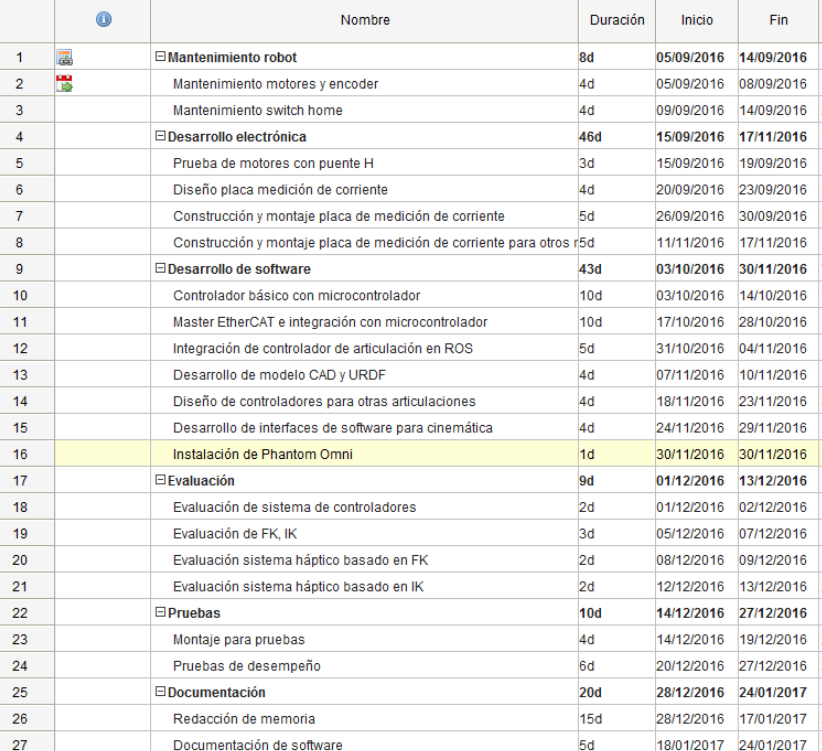
\includegraphics[scale=0.5]{img/cap1/tareas_gantt}
  \caption{Tareas en carta Gantt.}
  \label{cap1_tabla_gantt}
\end{figure}

Uno de los supuestos que presenta la planificación corresponde a que una vez desarrollado un controlador para una articulación, las otras articulaciones tendrán un tiempo de desarrollo mucho más acotado, pues se empleara el ya desarrollado como base.

Se espera que el desarrollo se inicie el 5 de septiembre de 2016 y concluya el 24 de enero de 2017, considerando tiempos de redacción de este documento y documentación asociada.








